%\documentclass[handout]{beamer}
%\documentclass[handout,10pt,slidestop,mathserif]{beamer}
%\usepackage{pgfpages}
%\pgfpagesuselayout{2 on 1}
\documentclass[10pt,slidestop,mathserif,c]{beamer}
\usetheme{Madrid}
\usecolortheme{seahorse}

\usepackage{tabularx}
\usepackage{verbatim}
\usepackage{graphics}
\usepackage{graphicx}
\usepackage[noae]{Sweave}
\usepackage{moreverb}
\usepackage{pgf}
\usepackage{tikz}
\usepackage{MnSymbol}
\usepackage[noae]{Sweave}


\newcommand{\putat}[3]{\begin{picture}(0,0)(0,0)\put(#1,#2){#3}\end{picture}}
  
\newenvironment{changemargin}[2]{%
  \begin{list}{}{%
    \setlength{\topsep}{0pt}%
    \setlength{\leftmargin}{#1}%
    \setlength{\rightmargin}{#2}%
    \setlength{\listparindent}{\parindent}%
    \setlength{\itemindent}{\parindent}%
    \setlength{\parsep}{\parskip}%
  }%
  \item[]}{\end{list}}

%% Define a new "leo" style for the package that will use a smaller font.
\makeatletter
\def\url@leostyle{%
  \@ifundefined{selectfont}{\def\UrlFont{\sf}}{\def\UrlFont{\tiny\ttfamily}}}
\makeatother

\title{Propensity Score Analysis with R}
\subtitle{Workshop for Division of Education of Educational Psychology \& Methodology, University at Albany}
\author[Bryer]{Jason M. Bryer \inst{1,2}\\\href{mailto:jason@bryer.org}{jason@bryer.org}}
\institute[Excelsior and UAlbany]{
  \begin{tabular}[h]{cc}
      \inst{1} Excelsior College &  \inst{2} University at Albany \\
      Albany, NY 12203 &  Albany, NY, 12222 \\
      \multicolumn{2}{c}{} \\
      \multicolumn{2}{c}{\url{http://github.com/jbryer/psa}}
  \end{tabular}      
}
\date[April 30 \& May 7, 2014]{April 30 \& May 7, 2014}

\begin{document}

%\AtBeginSection[]
%{
%   \begin{frame}
%       \frametitle{Agenda}
%       \tableofcontents[currentsection,currentsubsections]
%   \end{frame}
%}


\begin{frame}[plain]
  \titlepage
\end{frame}

%\frame{\frametitle{Agenda}\tableofcontents[hideothersubsections]}
\frame{\frametitle{Agenda}\tableofcontents}

%\AtBeginSubsection[]
%{
%\begin{frame}<beamer>{Agenda}
%\tableofcontents[currentsection,currentsubsection, 
% %   hideothersubsections, 
%    sectionstyle=show/shaded,
%]
%\end{frame}
%}

\begin{frame}
    \frametitle{Getting Started}
    \begin{itemize}
        \item All the course materials can be downloaded at \url{https://psa.bryer.org}. Click the "Download ZIP" button on the right side.
        \item You will need to download and install the following software:
        \begin{itemize}
            \item R: \url{http://cran.r-project.org}
            \item Rstudio: \url{http://www.rstudio.com}
            \item Rtools (Windows only): \url{http://cran.r-project.org/bin/windows/Rtools/}
        \end{itemize}

        \pause
        \ \\
        Other (shameless) plugs!

        \item Join the Albany R Users Group at \url{http://www.meetup.com/Albany-R-Users-Group/}
        \item I will be teaching EPSY 887 Data Science in the Fall \url{https://github.com/jbryer/EPSY887DataScience}
    \end{itemize}
        
    \pause
    
    \begin{center}\bf{Thanks to Hirah Mir and Heidi Andrade for making this workshop possible!}\end{center}
            
        
\end{frame}

\begin{frame}[containsverbatim,fragile]
    \frametitle{Popularity of Propensity Score Analysis}
    \begin{center}
        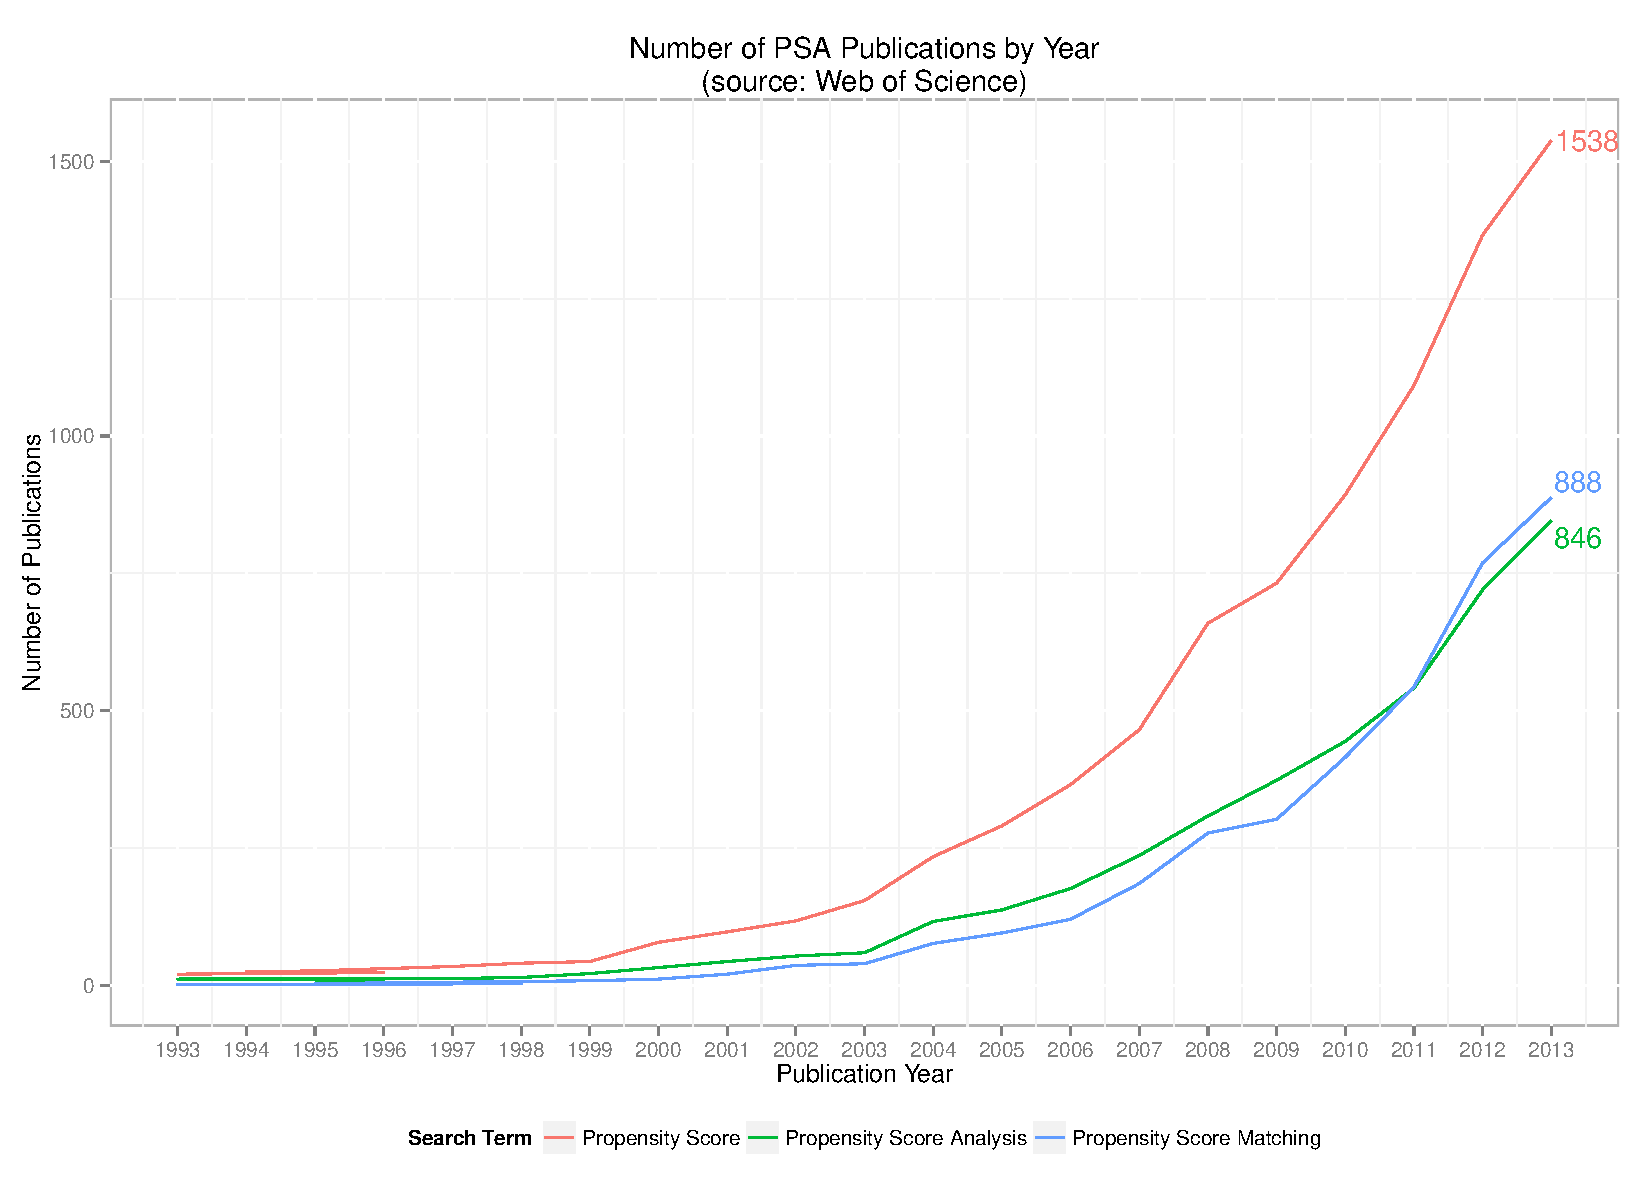
\includegraphics{figures/Slides-popularity}
    \end{center}
    
    %The number of publications for ``propensity score" has increase substantially over the last decade.

\end{frame}

%%%%%%%%%% Introduction

\section{Introduction to PSA (April 30, 2014)}

\subsection{Randomized Experiments}

\begin{frame}[containsverbatim,fragile]
    \frametitle{The Randomized Experiment}
    
    Considered to be the \textit{gold standard} for estimating causal effects.
    
    \begin{itemize}
        \item Effects can be estimated using simple means between groups, or blocks in randomized block design.
        \item Randomization presumes unbiasedness and balance between groups.
    \end{itemize}
    \ \\ \ \\
    However, randomization is often not feasible for many reasons, especially in educational contexts.
    \pause
    \ \\ \ \\
    The strong ignorability assumption states that:
    $$({ Y }_{ i }(1),{ Y }_{ i }(0)) \; \upModels \; { T }_{ i }|{ X }_{ i }=x$$
    for all ${X}_{i}$.
    
\end{frame}

\begin{frame}
    \frametitle{Rubin Causal Model\footnote{See Rubin, 1974, 1977, 1978, 1980, and Holland, 1986}}
    \begin{itemize}
        \item The causal effect of a treatment is the difference in an individual's outcome under the situation they were given the treatment and not (referred to as a counterfactual).
        $${\delta}_{i} ={ Y }_{ i1 }-{ Y }_{ i0 }$$
        \item However, it is impossible to directly observe ${\delta}_{i}$ (referred to as \textit{The Fundamental Problem of Causal Inference}, Holland 1986).
        \item Rubin frames this problem as a ``missing data problem."
    \end{itemize}
\end{frame}



\subsection{Defining Propensity Scores}

\begin{frame}
    \frametitle{Propensity Score Analysis}
    Propensity score analysis (PSA) is a quasi-experimental design used to estimate causal effects in observational studies (i.e. studies where students are not randomized to treatment). PSA is conducted in two phases:
    \begin{description}
        \item[Phase I] (Also referred to as the design phase) In phase one we are concerned with adjusting for selection bias. We model treatment placement using observed variables (see next slide). The propensity score is the probability of a student being in the treatment. With estimated propensity scores, clusters or matches are created for phase II.
        \item[Phase II] With matches or clusters made in phase I, we compare the difference between matches or clusters on the outcome measure of interest.
    \end{description}
\end{frame}


\begin{frame}[containsverbatim,fragile]
    \frametitle{Propensity Score Analysis}
    The propensity score is the "conditional probability of assignment to a particular treatment given a vector of observed covariates" (Rosenbaum \& Rubin, 1983, p. 41). The probability of being in the treatment:
    $$\pi ({ X }_{ i }) \; \equiv \; Pr({ T }_{ i }=1|{ X }_{ i })$$
    
    The balancing property under exogeneity:
    $${ T }_{ i } \; \upModels { X }_{ i } \;| \; \pi ({ X }_{ i })$$
    
    We can then restate the ignorability assumption with the propensity score: 
    $$({ Y }_{ i }(1),{ Y }_{ i }(0)) \; \upModels \; { T }_{ i } \; | \; \pi({ X }_{ i })$$
\end{frame}
    
\begin{frame}[containsverbatim,fragile]
    \frametitle{Treatment Effects}    
    The average treatment effect (ATE) is defined as:
    $$E({ r }_{ 1 })-E({ r }_{ 0 })$$
    where $E(.)$ is the expectation in the population. For a set of covariates, $X$, and outcomes $Y$ where 0 denotes control and 1 treatment, we define ATE as:
    $$ATE=E(Y_{1}-Y_{0}|X)=E(Y_{1}|X)-E(Y_{0}|X)$$
    The Average treatment effect on the treated (ATT), is defined as:
    $$ATT=E(Y_{1}-Y_{0}|X,C=1)=E(Y_{1}|X,C=1)-E(Y_{0}|X,C=1)$$
\end{frame}

\subsection{Different Methods of PSA}

\begin{frame}
    \frametitle{Propensity score methods}
    \begin{description}
        \item[Matching] Each treatment unit is paired with a comparison unit based upon the pre-treatment covariates.
        \item[Stratification] Treatment and comparison units are divided into strata (or subclasses) so that treated and comparison units are similar within each strata. Cochran (1968) observed that creating five subclassifications (stratum) removes at least 90\% of the bias in the estimated treatment effect.
        \item[Weighting] Each observation is weighted by the inverse of the probability of being in that group.
        $$\frac { 1 }{ n } \sum _{ i=1 }^{ n }{ \left( \frac { { T }_{ i }{ Y }_{ i } }{ \pi ({ X }_{ i }) } -\frac { (1-{ T }_{ i }){ Y }_{ i } }{ 1-\pi ({ X }_{ i }) }  \right)  } $$
    \end{description}

\end{frame}

\begin{frame}[containsverbatim,fragile]
    \frametitle{Steps for Implementing Matching Methods}
    Stuart and Rubin (2008) outline the following steps for matching, but the same approach can be used for stratification and weighting as well.
    \begin{enumerate}
        \item Choose the covariates to be used.
        \item Define a distance measure (i.e. what constitutes similar).
        \item Choose the matching algorithm.
        \item Diagnose the matches (or strata) obtained (iterating through steps 2 and 3 as well).
        \item Estimate the treatment effect using the matches (or strata) found in step 4.
    \end{enumerate}

\end{frame}


\begin{frame}[containsverbatim,fragile]
    \frametitle{Matching Methods}
    There are many choices and approaches to matching, including:
    \begin{itemize}
        \item Propensity score matching.
        \item Limited exact matching.
        \item Full matching.
        \item Nearest neighbor matching.
        \item Optimal/Genetic matching.
        \item Mahalanobis distance matching (for quantiative covariates only).
%        $$\sqrt { { \left( { X }_{ i }-{ X }_{ j } \right)  }^{ T }{ S }^{ -1 }\left( { X }_{ i }-{ X }_{ j } \right)  } $$ where S is the covariance matrix.
        \item Matching with and without replacement.
        \item One-to-one or one-to-many matching.
    \end{itemize}
    \ \\
    Which matching method should you use?
    \pause
    \begin{center} \textbf{Whichever one gives the best balance!} \end{center}
    See Rosenbaum (2012), \textit{Testing one hypothesis twice in observational studies}.
\end{frame}

\subsection{The Lalonde Example}

\begin{frame}[containsverbatim,fragile]
    \frametitle{National Supported Work}
    
    The National Supported Work (NSW) Demonstration was a federally and privately funded randomized experiment done in the 1970s to estimate the effects of a job training program for disadvantaged workers.
    
    \begin{itemize}
        \item Participants were randomly selected to participate in the training program.
        \item Both groups were followed up to determine the effect of the training on wages.
        \item Analysis of the mean differences (unbiased given randomization), was approximately \$800.
    \end{itemize}
    
    Lalonde (1986) used data from the Panel Survey of Income Dynamics (PSID) and the Current Population Survey (CPS) to investigate whether non-experimental methods would result in similar results to the randomized experiment. He found results ranging from \$700 to \$16,000.
\end{frame}

\begin{frame}[containsverbatim,fragile]
    \frametitle{National Supported Work (cont.)}
    Dehejia and Wahba (1999) later used propensity score matching to analyze the data. The found that,
    \begin{itemize}
        \item Comparison groups selected by Lalonde were very dissimilar to the treated group.
        \item By restricting the comparison group to those that were similar to the treated group, they could replicate the original NSW results.
        \item Using the CPS data, the range of treatment effect was between \$1,559 to \$1,681. The experimental results for the sample sample was approximately \$1,800.
    \end{itemize}

    The covariates available include: age, eduction level, high school degree, marital status, race, ethnicity, and earning sin 1974 and 1975.
    \ \\ \ \\
    Outcome of interest is earnings in 1978.
    
\begin{Schunk}
\begin{Sinput}
> data(lalonde, package='Matching')
\end{Sinput}
\end{Schunk}
\end{frame}


\begin{frame}[containsverbatim,fragile,shrink=.8]
    \frametitle{Estimating Propensity Scores}
\begin{Schunk}
\begin{Sinput}
> lalonde.formu <- treat~age + educ  + black + hisp + married + nodegr + re74 + re75
> glm1 <- glm(lalonde.formu, family=binomial, data=lalonde)
> summary(glm1)
\end{Sinput}
\begin{Soutput}
Call:
glm(formula = lalonde.formu, family = binomial, data = lalonde)

Deviance Residuals: 
   Min      1Q  Median      3Q     Max  
-1.436  -0.990  -0.907   1.282   1.695  

Coefficients:
             Estimate Std. Error z value Pr(>|z|)   
(Intercept)  1.18e+00   1.06e+00    1.12    0.265   
age          4.70e-03   1.43e-02    0.33    0.743   
educ        -7.12e-02   7.17e-02   -0.99    0.321   
black       -2.25e-01   3.66e-01   -0.61    0.539   
hisp        -8.53e-01   5.07e-01   -1.68    0.092 . 
married      1.64e-01   2.77e-01    0.59    0.555   
nodegr      -9.04e-01   3.13e-01   -2.88    0.004 **
re74        -3.16e-05   2.58e-05   -1.22    0.221   
re75         6.16e-05   4.36e-05    1.41    0.157   
---
Signif. codes:  0 '***' 0.001 '**' 0.01 '*' 0.05 '.' 0.1 ' ' 1

(Dispersion parameter for binomial family taken to be 1)

    Null deviance: 604.20  on 444  degrees of freedom
Residual deviance: 587.22  on 436  degrees of freedom
AIC: 605.2

Number of Fisher Scoring iterations: 4
\end{Soutput}
\end{Schunk}
\end{frame}


\subsection{Matching}

\begin{frame}[containsverbatim,fragile]
    \frametitle{Estimating Propensity Scores}
\begin{Schunk}
\begin{Sinput}
> ps <- fitted(glm1)  # Propensity scores
> Y  <- lalonde$re78  # Dependent variable, real earnings in 1978
> Tr <- lalonde$treat # Treatment indicator
> rr <- Match(Y=Y, Tr=Tr, X=ps, M=1, ties=FALSE)
> summary(rr) # The default estimate is ATT here
\end{Sinput}
\begin{Soutput}
Estimate...  2726.3 
SE.........  633.85 
T-stat.....  4.3011 
p.val......  1.6992e-05 

Original number of observations..............  445 
Original number of treated obs...............  185 
Matched number of observations...............  185 
Matched number of observations  (unweighted).  185 
\end{Soutput}
\end{Schunk}
\end{frame}

\begin{frame}[containsverbatim,fragile]
    \frametitle{Visualizing Results}
\begin{Schunk}
\begin{Sinput}
> matches <- data.frame(Treat=lalonde[rr$index.treated,'re78'], 
   Control=lalonde[rr$index.control,'re78'])
> print(granovagg.ds(matches))
\end{Sinput}
\begin{Soutput}
                              Summary Statistics
n                                        1.8e+02
Treat mean                               6.3e+03
Control mean                             3.6e+03
mean(D = Treat - Control)                2.7e+03
SD(D)                                    8.6e+03
Effect Size                              3.2e-01
r(Treat, Control)                        5.4e-02
r(Treat + Control, D)                    5.8e-01
Lower 95% Confidence Interval            1.5e+03
Upper 95% Confidence Interval            4.0e+03
t (D-bar)                                4.3e+00
df.t                                     1.8e+02
p-value (t-statistic)                    0.0e+00
\end{Soutput}
\end{Schunk}
\end{frame}

\begin{frame}[containsverbatim,fragile]
    \begin{center}
        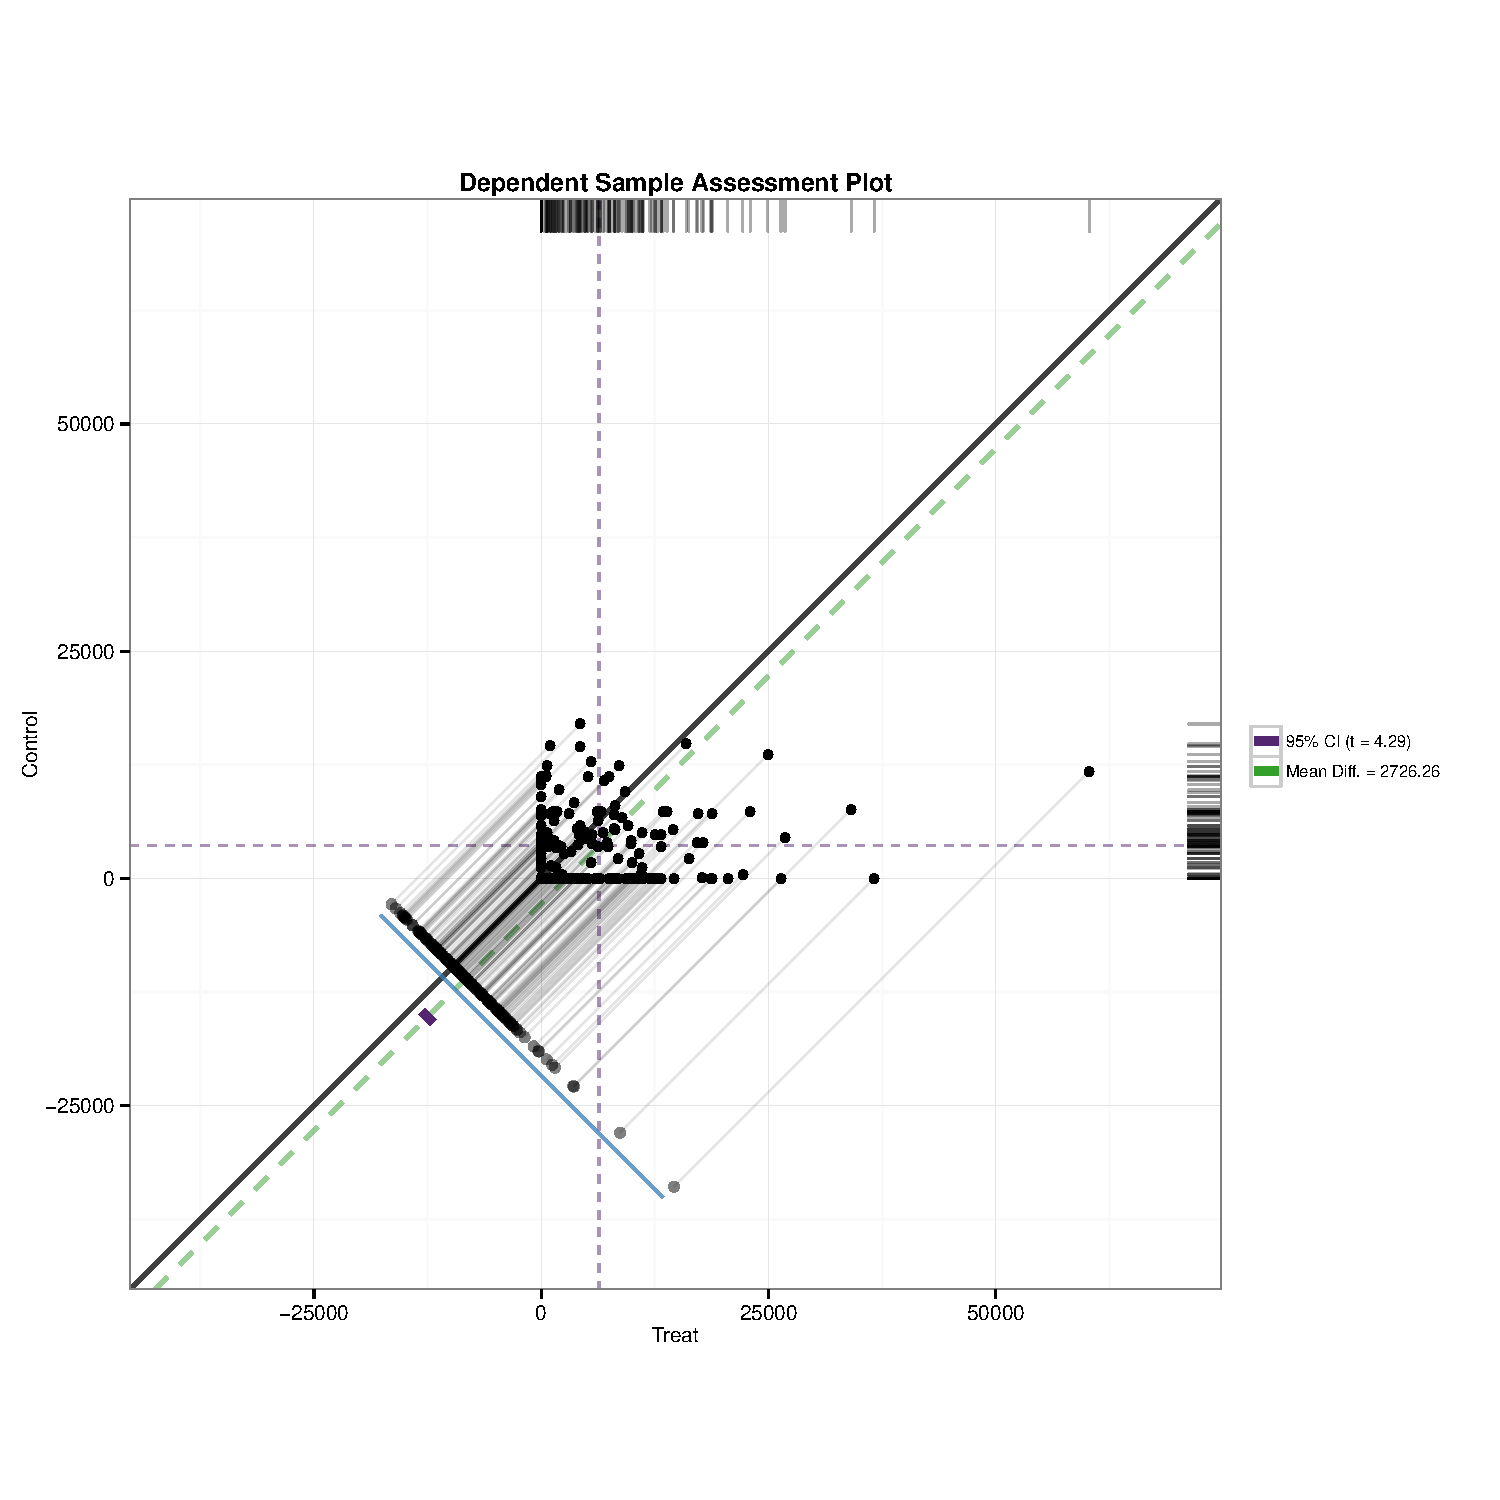
\includegraphics{figures/Slides-granovaggds}
    \end{center}
\end{frame}

%%%%% Stratification
\subsection{Stratification}

\begin{frame}[containsverbatim,fragile,shrink=.8]
    \frametitle{Stratification (5 Strata)}
\begin{Schunk}
\begin{Sinput}
> strata <- cut(ps, quantile(ps, seq(0, 1, 1/5)), include.lowest=TRUE, labels=letters[1:5])
> circ.psa(lalonde$re78, lalonde$treat, strata, revc=TRUE)
\end{Sinput}
\begin{Soutput}
$summary.strata
  n.0 n.1 means.0 means.1
a  62  27    5126    5178
b  59  30    3855    6497
c  56  33    4587    4495
d  42  47    4814    6059
e  41  48    4388    8474

$wtd.Mn.1
[1] 6141

$wtd.Mn.0
[1] 4554

$ATE
[1] -1587

$se.wtd
[1] 694

$approx.t
[1] -2.3

$df
[1] 435

$CI.95
[1] -2950  -224
\end{Soutput}
\end{Schunk}
\end{frame}

\begin{frame}[containsverbatim,fragile]
    \frametitle{Stratification (5 Strata)}
    \begin{center}
        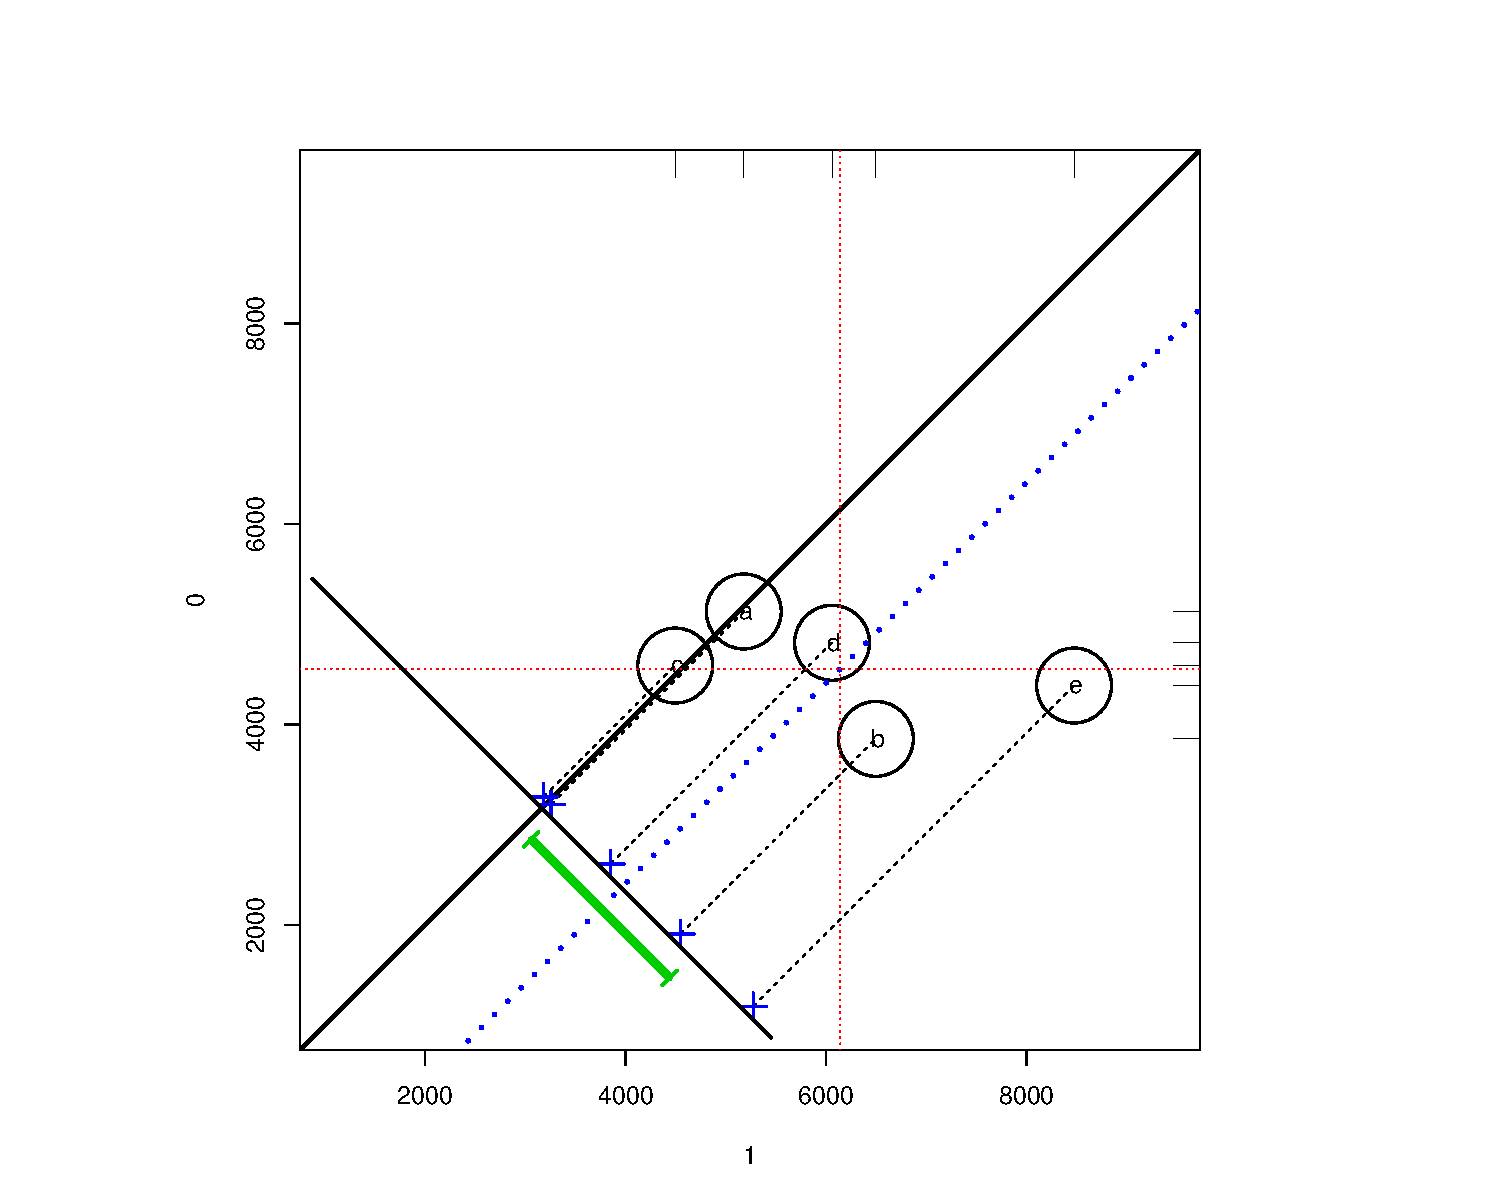
\includegraphics{figures/Slides-circpsa5}
    \end{center}    
\end{frame}


\begin{frame}[containsverbatim,fragile,shrink=.8]
    \frametitle{Stratification (10 Strata)}
\begin{Schunk}
\begin{Sinput}
> strata10 <- cut(ps, quantile(ps, seq(0, 1, 1/10)), include.lowest=TRUE, labels=letters[1:10])
> circ.psa(lalonde$re78, lalonde$treat, strata10, revc=TRUE)
\end{Sinput}
\begin{Soutput}
$summary.strata
  n.0 n.1 means.0 means.1
a  35  10    6339    7020
b  27  17    3554    4095
c  31  16    3430    4357
d  28  14    4326    8943
e  30  15    4933    4711
f  26  18    4188    4315
g  22  22    4755    6149
h  20  25    4879    5980
i  16  28    1375    9276
j  25  20    6316    7351

$wtd.Mn.1
[1] 6195

$wtd.Mn.0
[1] 4414

$ATE
[1] -1781

$se.wtd
[1] 711

$approx.t
[1] -2.5

$df
[1] 425

$CI.95
[1] -3178  -384
\end{Soutput}
\end{Schunk}
\end{frame}

\begin{frame}[containsverbatim,fragile]
    \frametitle{Stratification (10 Strata)}
    \begin{center}
        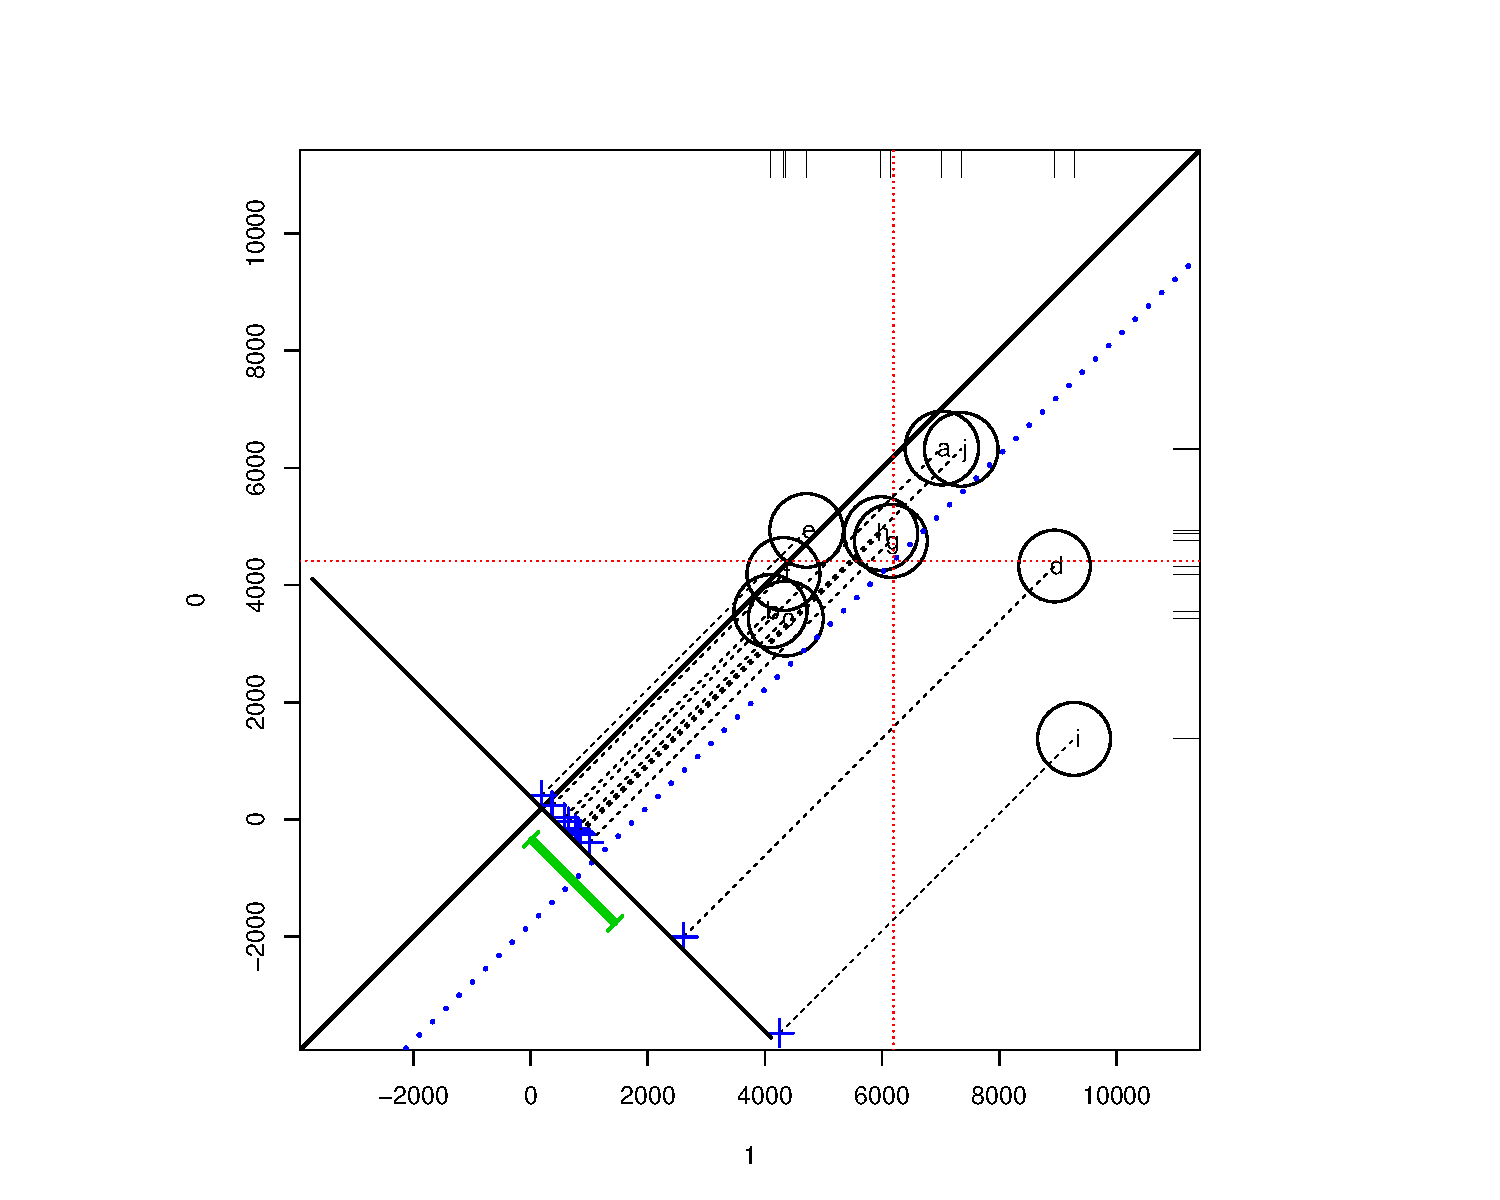
\includegraphics{figures/Slides-circpsa10}
    \end{center}    
\end{frame}


\begin{frame}[containsverbatim,fragile,shrink=.8]
    \frametitle{Loess Regression}
    \begin{center}
        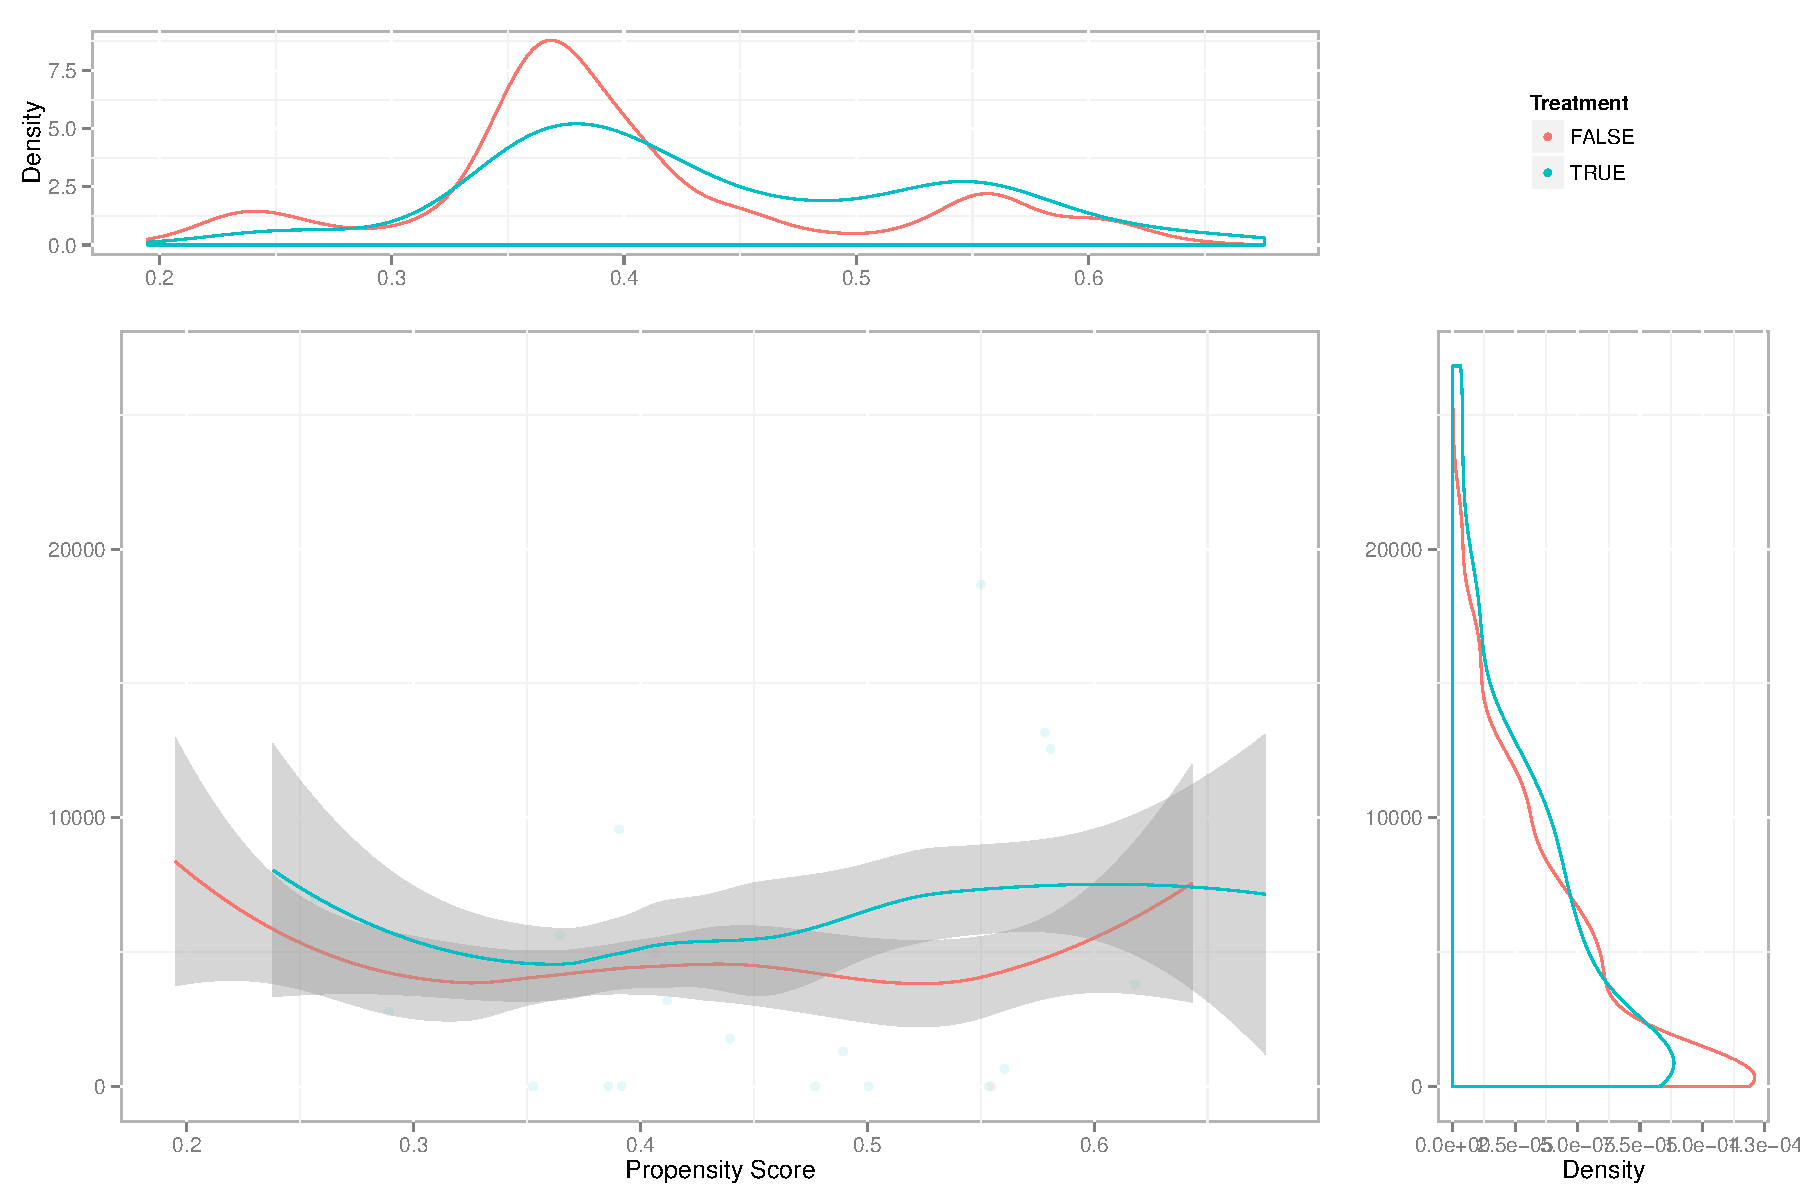
\includegraphics{figures/Slides-loessplot}
    \end{center}    
\end{frame}


%%%%% Checking Balance

\begin{frame}[containsverbatim,fragile]
    \frametitle{Checking Balance: Continuous Covariates}
\begin{Schunk}
\begin{Sinput}
> box.psa(lalonde$age, lalonde$treat, strata, xlab="Strata", 
   balance=FALSE)
\end{Sinput}
\end{Schunk}
    \begin{center}
        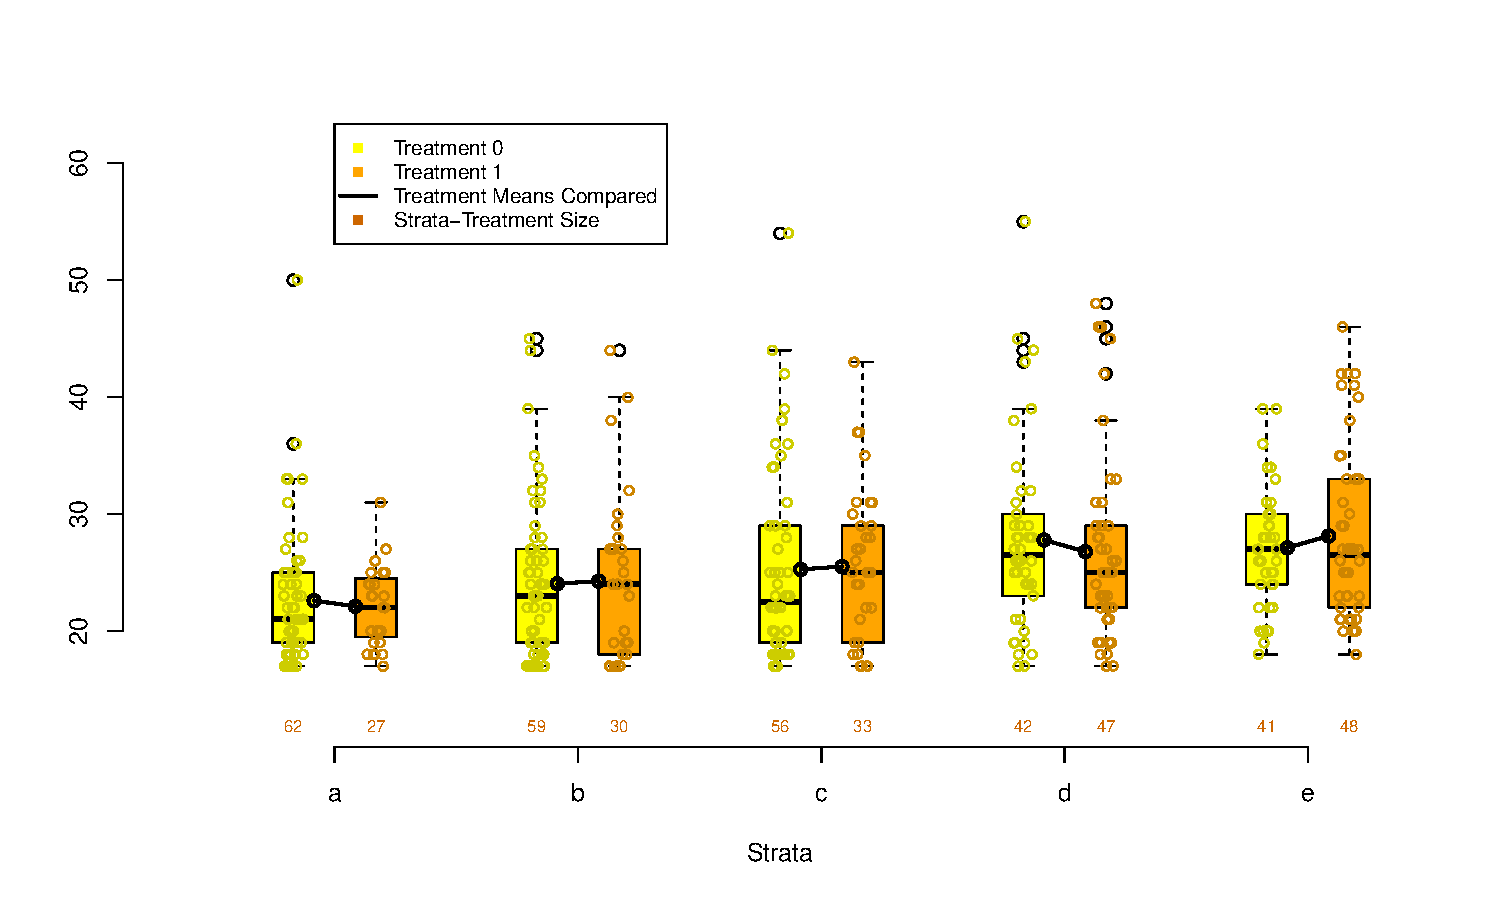
\includegraphics{figures/Slides-boxpsa}
    \end{center}
\end{frame}

\begin{frame}[containsverbatim,fragile]
    \frametitle{Checking Balance: Categorical Covariates}
\begin{Schunk}
\begin{Sinput}
> cat.psa(lalonde$married, lalonde$treat, strata, xlab='Strata', 
   balance=FALSE)
\end{Sinput}
\end{Schunk}
    \begin{center}
        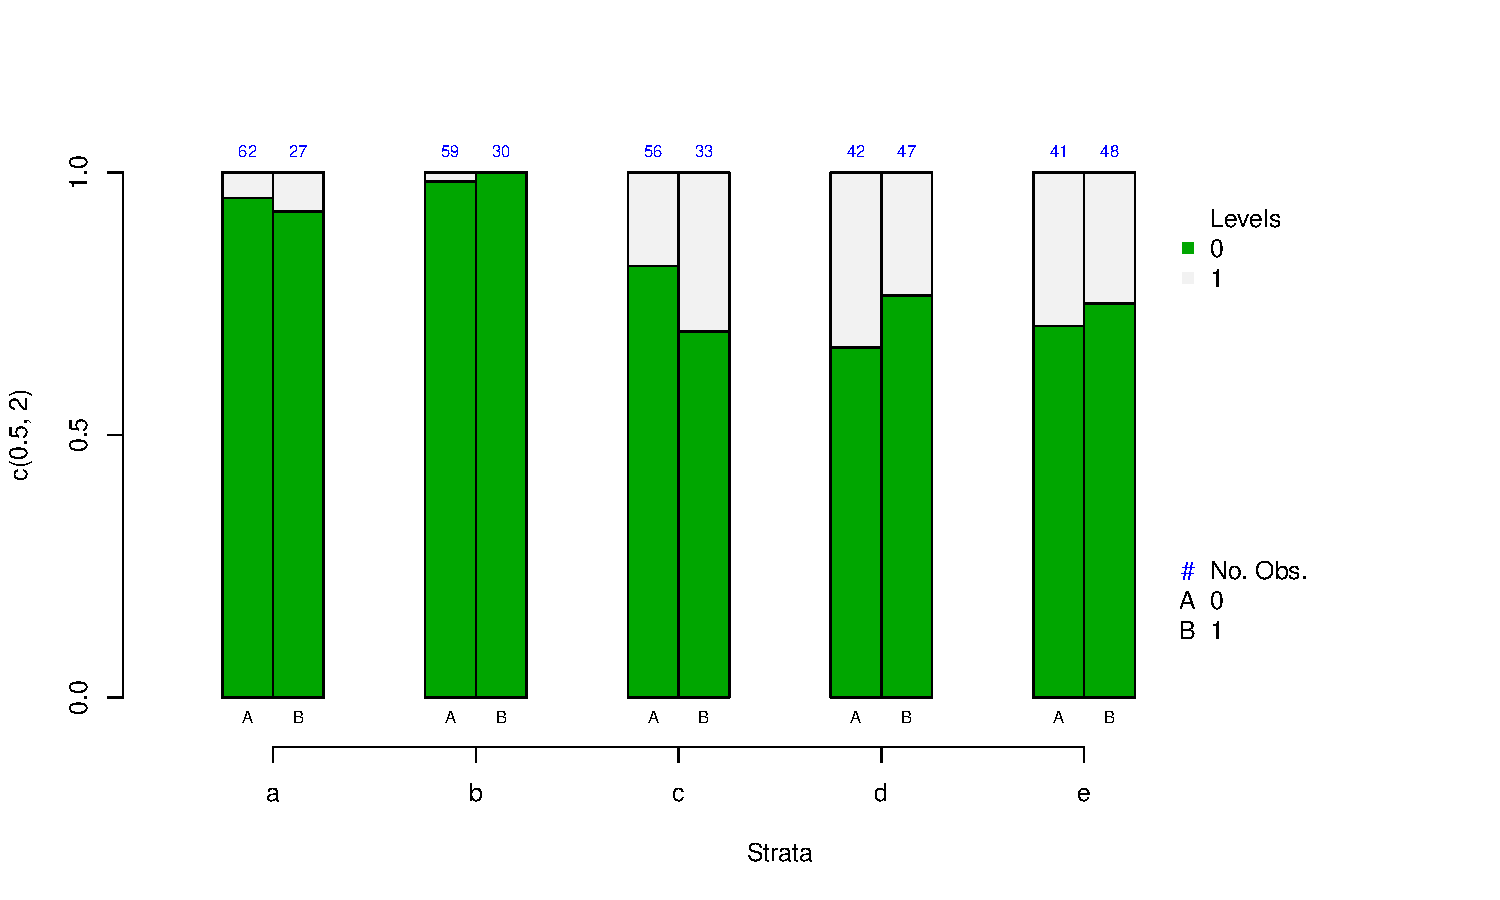
\includegraphics{figures/Slides-catpsa}
    \end{center}
\end{frame}

\begin{frame}[containsverbatim,fragile]
    \frametitle{Checking Balance: Covariate Balance Plot}
    \begin{center}
        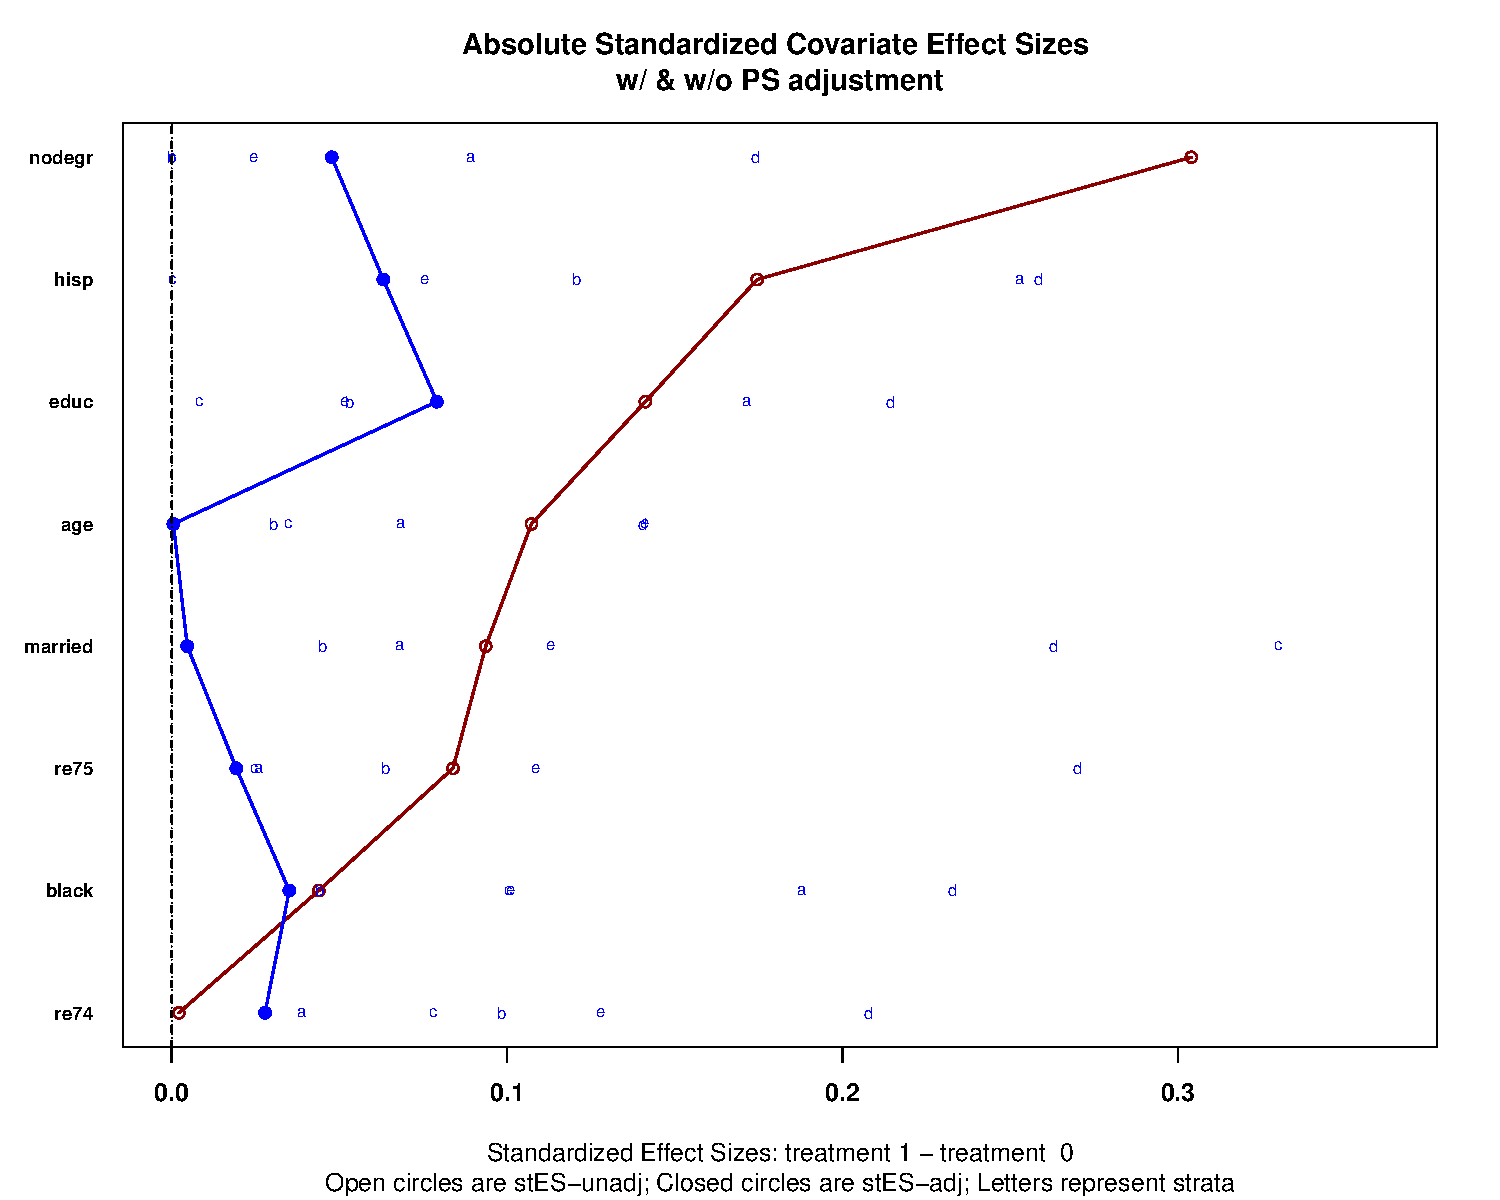
\includegraphics{figures/Slides-cvbalpsa}
    \end{center}
\end{frame}


%%%%%%%%%%%%%%%%%%%%%%%%%%%%%%%%%%%%%%%%%%%%%%%%%%%%%%%%%%%%%%%%%%%%%%%%%%%%%%%%%%%%%%%%%%
\section{Advanced PSA (May 7, 2014)}

%%%%%%%%%%%%%%%%%%%%%%%%%%%%%%%%%%%%%%%%%%%%%%%%%%%%%%%%%%%%%%%%%%%%%%%%%%%%%%%%%%%%%%%%%%
\subsection{Sensitivity Analysis}


%%%%%%%%%%%%%%%%%%%%%%%%%%%%%%%%%%%%%%%%%%%%%%%%%%%%%%%%%%%%%%%%%%%%%%%%%%%%%%%%%%%%%%%%%%
\subsection{Missing Data}


%%%%%%%%%%%%%%%%%%%%%%%%%%%%%%%%%%%%%%%%%%%%%%%%%%%%%%%%%%%%%%%%%%%%%%%%%%%%%%%%%%%%%%%%%%
\subsection{Bootstrapping}


%%%%%%%%%%%%%%%%%%%%%%%%%%%%%%%%%%%%%%%%%%%%%%%%%%%%%%%%%%%%%%%%%%%%%%%%%%%%%%%%%%%%%%%%%%
\subsection{Matching of Non-Binary Treatments}



\begin{frame}[containsverbatim,fragile]
    \frametitle{Matching of Non-Binary Treatments}
    
    \begin{itemize}
        \item The \texttt{TriMatch} package provides functions for finding matched triplets.
        \item Estimates propensity scores for three separate logistic regression models (one for each pair of groups, that is, treat1-to-control, treat2-to-control, and treat1-to-treat2).
        \item Finds matched triplets that minimize the total distance (i.e. sum of the standardized distance between propensity scores within the three modesl). within a caliper.
        \item Provides multiple methods for determining which matched triplets are retained:
            \begin{itemize}
                \item Optimal which attempts to retain all treatment units.
                \item Full which retains all matched triplets within the specified caliper (.25 by default as suggested by Rosenbaum).
                \item Analog of the one-to-many for matched triplets. Specify how many times each treat1 and treat2 unit can be matched.
                \item Unique which allows each unit to be matched once, and only once.
            \end{itemize}
        \item Functions for conducting repeated measures ANOVA and Freidman Ranksum Tests are provided.
    \end{itemize}
\end{frame}

\begin{frame}
    \frametitle{Example: Tutoring}
    Students can opt to utilize tutoring services to supplement math courses. Of those who used tutoring services, approximately 58\% of students used the tutoring service once, whereas the remaining 42\% used it more than once. Outcome of interest is course grade.
    \begin{description}
        \item[Military] Active military status.
        \item[Income] Income level.
        \item[Employment] Employment level.
        \item[NativeEnglish] Is English their native language
        \item[EdLevelMother] Education level of their mother.
        \item[EdLevelFather] Education level of their father.
        \item[Ethnicity] American Indian or Alaska Native, Asian, Black or African American, Hispanic, Native Hawaiian or Other Pacific Islander, Two or more races, Unknown, White
        \item[Gender] Male, Female
        \item[Age] Age at course start.
        \item[GPA] Student GPA at the beginning of the course.
    \end{description}

\end{frame}

%\begin{frame}
%    \frametitle{New Student Outreach: Covariates}
%    Newly enrolled students received outreach contacts until they registered for a course or six months have passed, whichever came first. Outreach was conducted by two academic advisors and a comparison group was drawn from students who enrolled prior to the start of the outreach program. Outcome of interest is number of credits attempted within the first seven months of enrollment.
%    \begin{description}
%        \item[Military] Active military status.
%        \item[Income] Income level.
%        \item[Employment] Employment level.
%        \item[NativeEnglish] Is English their native language: Yes (345), No (29)
%        \item[EdLevelMother] Education level of their mother.
%        \item[EdLevelFather] Education level of their father.
%        \item[Ethnicity] American Indian or Alaska Native, Asian, Black or African American, Hispanic, Native Hawaiian or Other Pacific Islander, Two or more races, Unknown, White
%        \item[Gender] Male (109), Female (265)
%        \item[Age] Age (mean=35.5, SD=9.7)
%    \end{description}
%
%\end{frame}


\begin{frame}[containsverbatim,fragile]
    \frametitle{PSA for Non-Binary Treatments}
    \begin{itemize}
        \item The \texttt{TriMatch} algorithm works as follows:
        \begin{enumerate}
            \item Estimate three separate propensity score models for each pair of groups (i.e. Control-to-Treat1, Control-to-Treat2, Treat1-to-Treat2).
            \item Determine the matching order. The default is to start with the largest of two treatments, then the other treatment, followed by the control.
            \item For each unit in group 1, find all units from group 2 within a certain threshold (i.e. difference between PSs is within a specified caliper).
            \item For each unit in group 2, find all units from group 3 within a certain threshold.
            \item Calculate the distance (difference) between each unit 3 found and the original unit 1. Eliminate candidates that exceed the caliper.
            \item Calculate a total distance (sum of the three distances) and retain the smallest unique \textit{M} group 1 units (by default \textit{M}=2)
        \end{enumerate}
    \end{itemize}
\end{frame}


\begin{frame}[containsverbatim,fragile]
    \frametitle{Matching Triplets} 
\begin{center}
    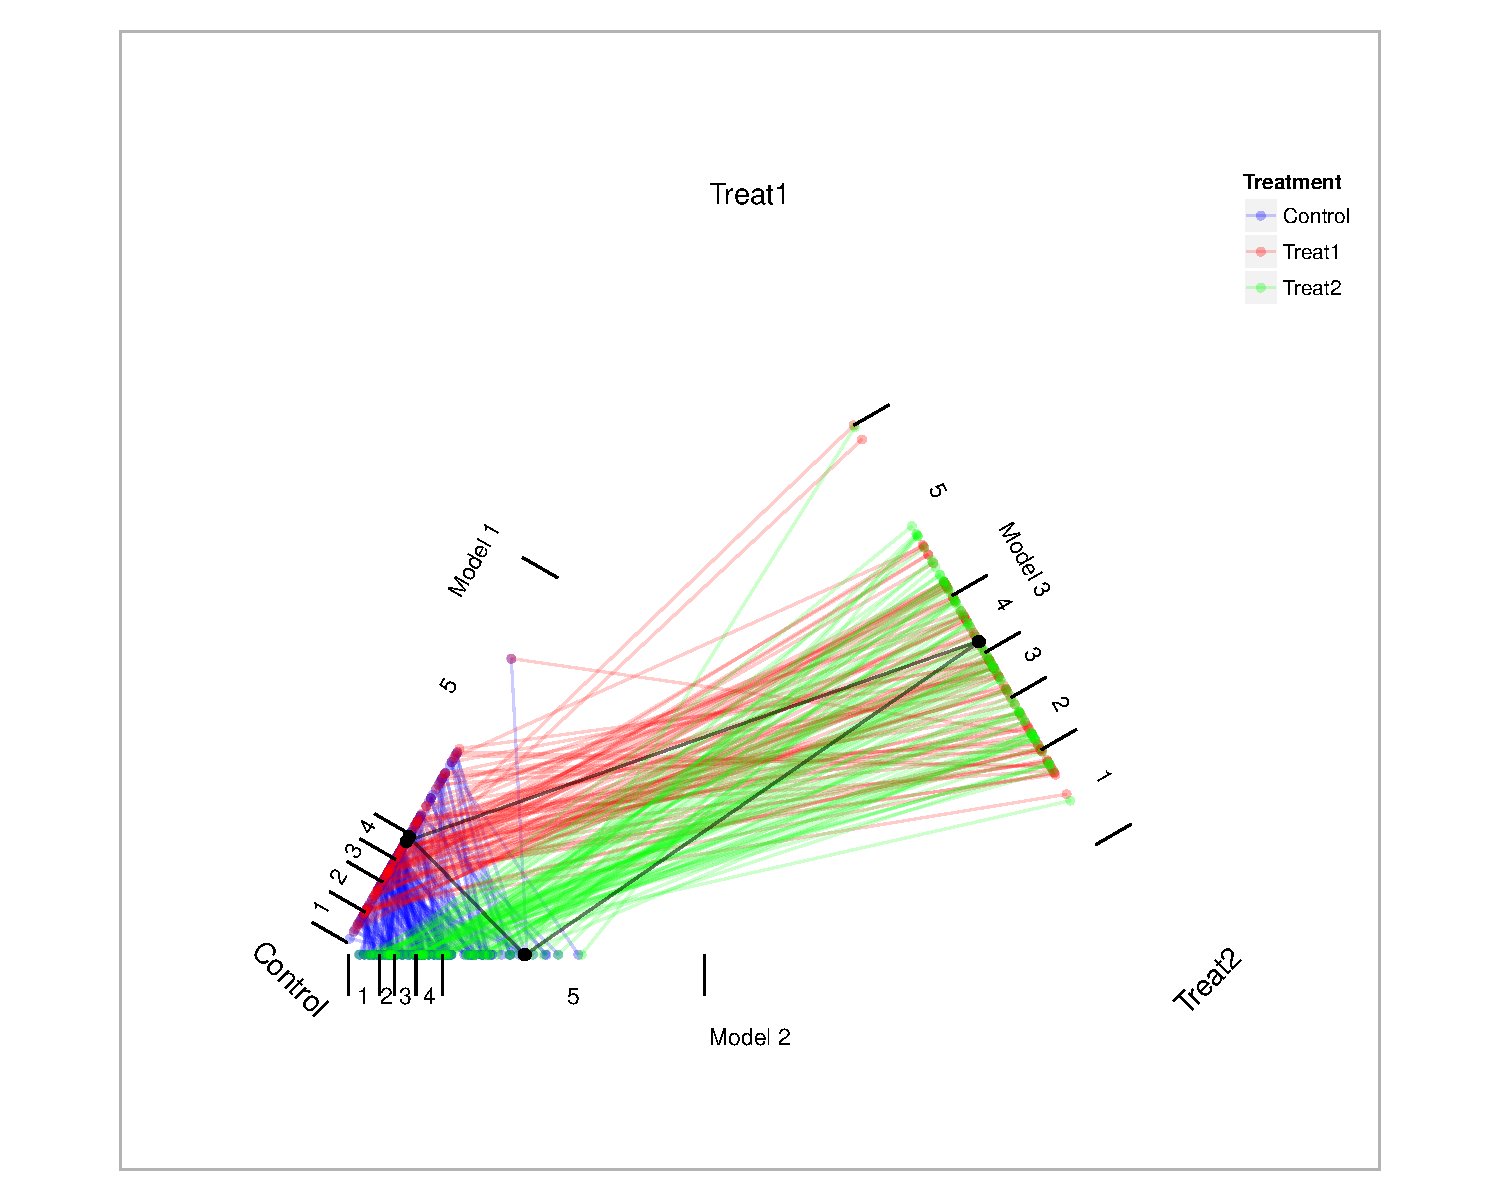
\includegraphics{figures/Slides-triangleplot}
\end{center}

\end{frame}

\begin{frame}[containsverbatim,fragile]
    \frametitle{Checking Balance}
\begin{center}
    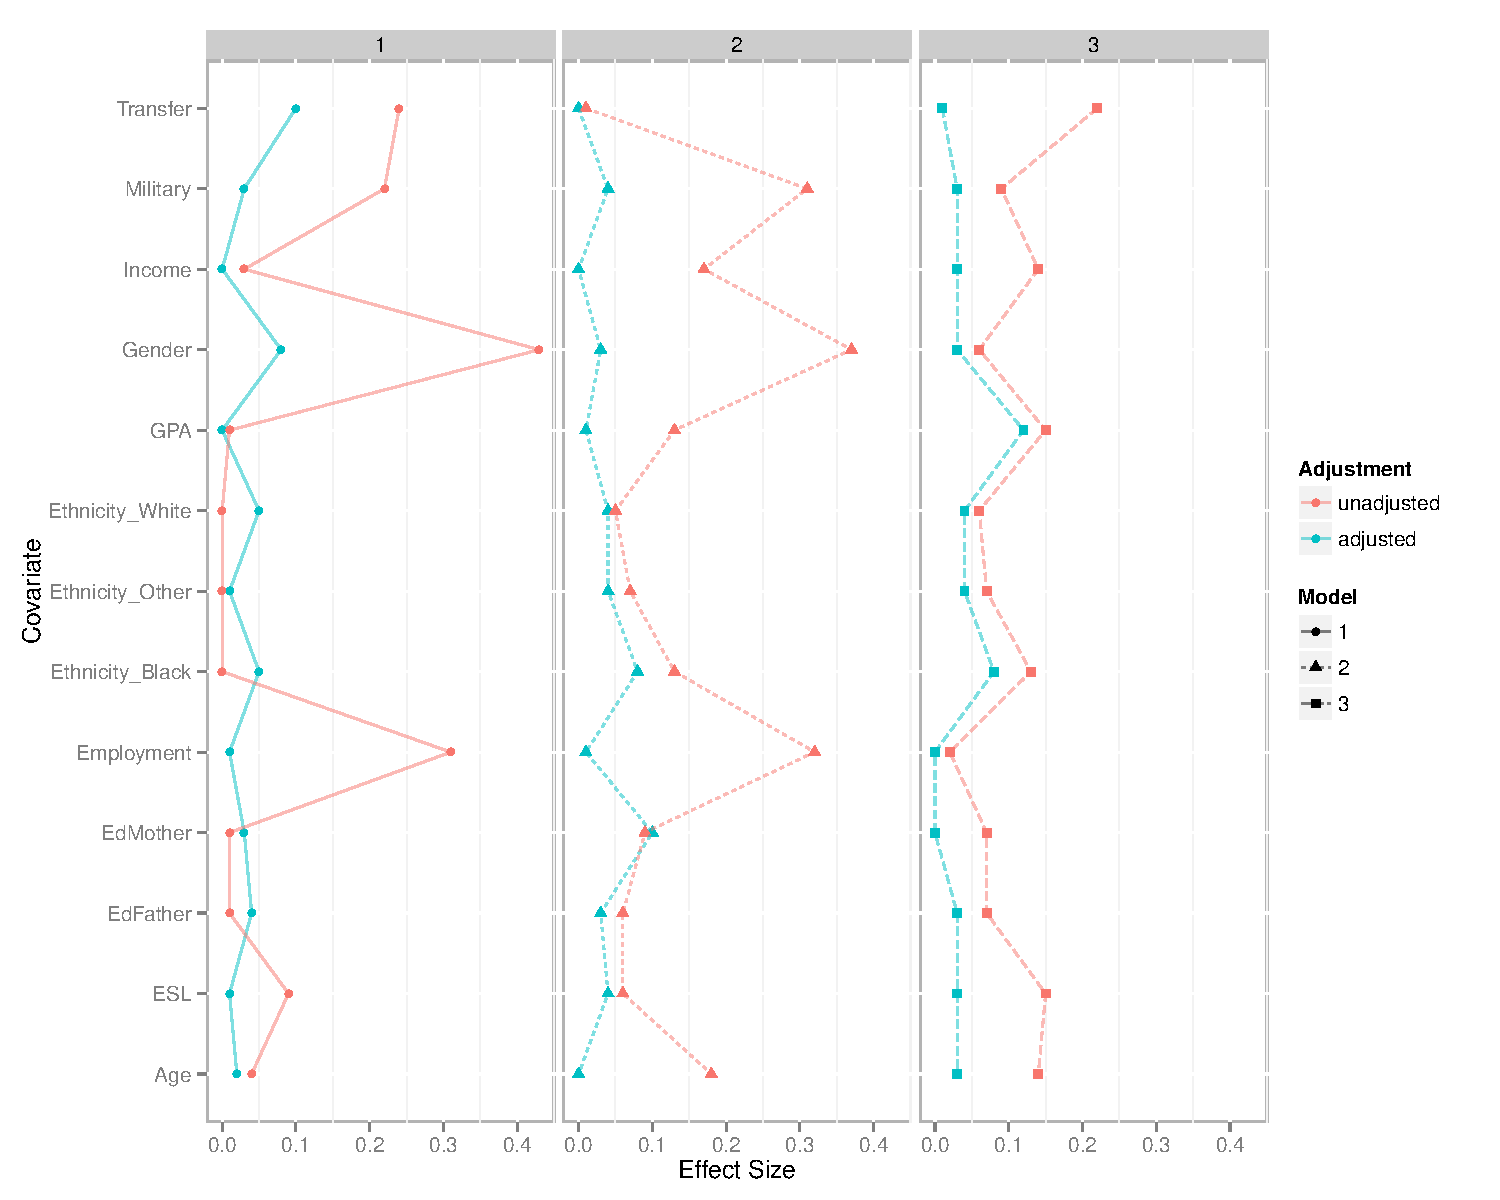
\includegraphics{figures/Slides-balanceplot}
\end{center}
\end{frame}

\begin{frame}[containsverbatim,fragile]
    \frametitle{Results}
\begin{center}
    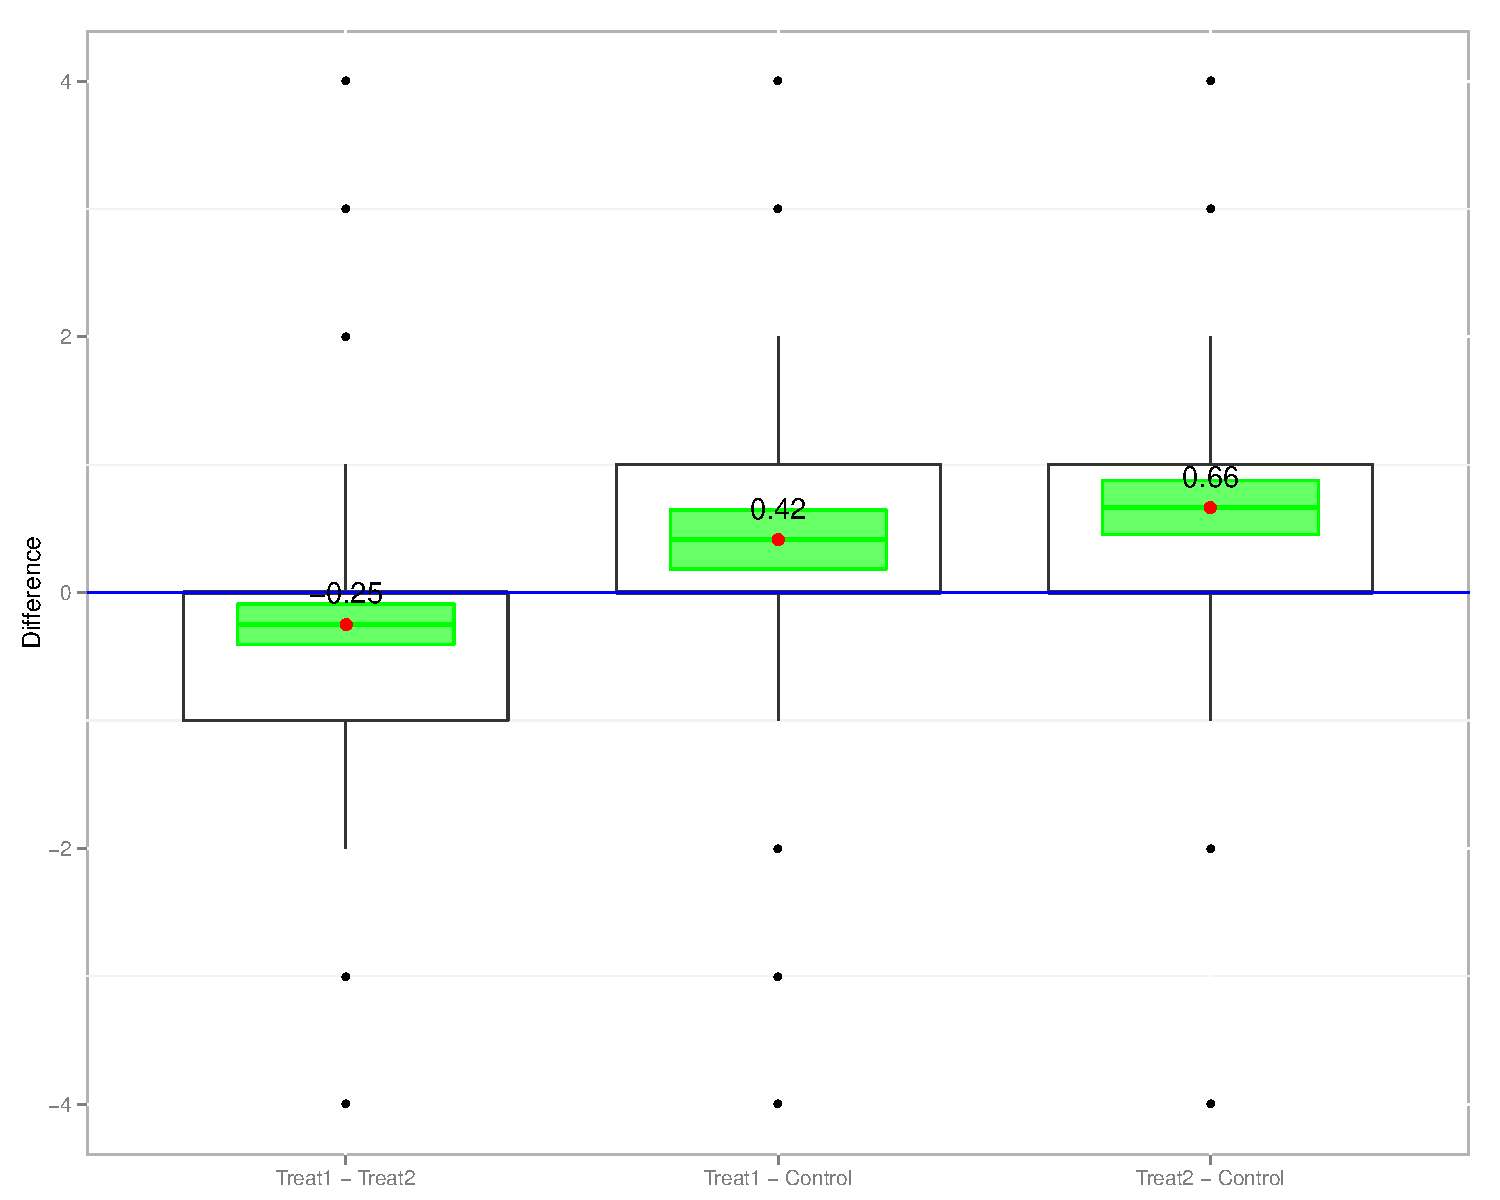
\includegraphics{figures/Slides-boxdiff}
\end{center}
\end{frame}


%%%%%%%%%% Multilevel PSA
\subsection{Multilevel PSA}

\begin{frame}[containsverbatim,fragile]
    \frametitle{Multilevel PSA}
    The use of PSA for clustered, or multilevel data, has been limited (Thoemmes \& Felix, 2011). Bryer and Pruzek (2012, 2013) have introduced an approach to analyzing multilevel or clustered data using stratification methods and implemented in the \texttt{multilevelPSA} R package.
    \begin{itemize}
        \item Exact and partially exact matching methods implicitly adjust for clustering. That is, the covariates chosen to exactly match are, in essence, clustering variables.
        \item Exact matching only applies to phase I of PSA. How are the clusters related to outcome of interest.
    \end{itemize}  
    The \texttt{multilevelPSA} uses stratification methods (e.g. quintiles, classification trees) by:
    \begin{itemize}
        \item Estimate separate propensity scores for each cluster.
        \item Identify strata within each cluster (e.g. leaves of classification trees, quintiles).
        \item Estimate ATE (or ATT) within each cluster.
        \item Aggregate estimated ATE to provide an overall ATE estimate.
        \item Several functions to summarize and visualize results and check balance.
    \end{itemize}
\end{frame}

\begin{frame}[containsverbatim,fragile]
    \frametitle{The Programme of International Student Assessment (PISA)}
    \begin{itemize}
        \item International assessment conducted by the Organization for Economic Co-operation and Development (OECD).
        \item Assesses students towards the end of secondary school (approximately 15-year-old children) in math, reading, and science.
        \item Collects a robust set of background information from students, parents, teachers, and schools.
        \item Assess both private and public school students in many countries.
        \item We will use PISA to estimate the effects of private school attendance on PISA outcomes.
    \end{itemize}
\end{frame}


\begin{frame}[containsverbatim,fragile]
    \frametitle{Phase I of Multilevel PSA}
    The \texttt{multilevelPSA} provides two functions, \texttt{mlpsa.ctree} and \texttt{mlpsa.logistic}, that will estimate propensity scores using classification trees and logistic regression, respectively. Since logistic regression requires a complete dataset (i.e. no missing values), we will use classification trees in this example.
\begin{Schunk}
\begin{Sinput}
> data(pisana)
> data(pisa.colnames)
> data(pisa.psa.cols)
> student = pisana
> mlctree = mlpsa.ctree(student[,c('CNT','PUBPRIV',pisa.psa.cols)], 
   					  formula=PUBPRIV ~ ., level2='CNT')